\begin{tikzpicture}
	%\node[inner sep=0pt] (A) at (1,4)
	%{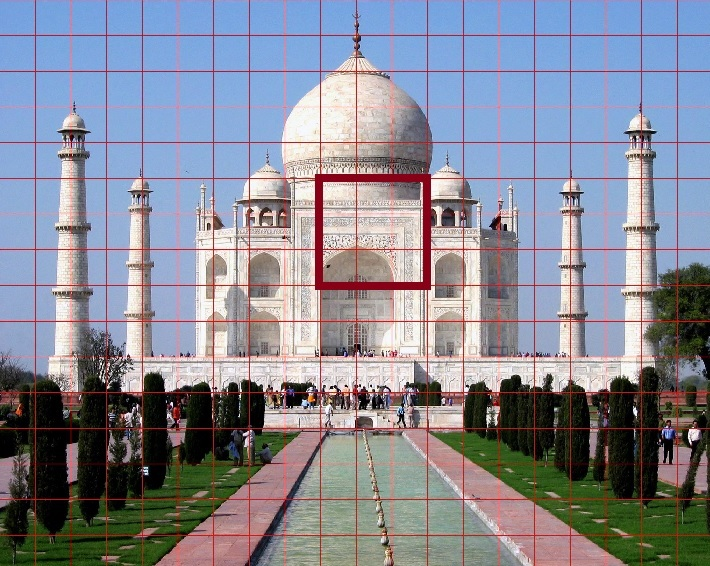
\includegraphics[width=5cm,height=5cm]     {images/CNN}};
	
	\onslide<1->{  \node[inner sep=0pt] (A) at (3,6.5)
		{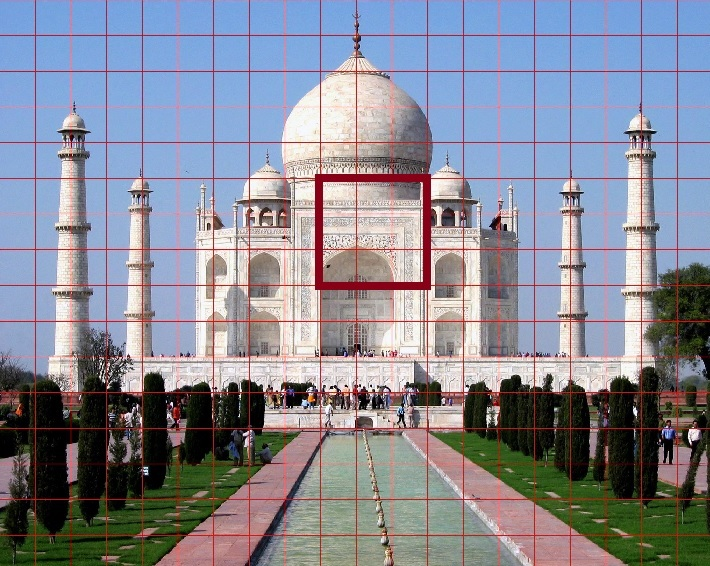
\includegraphics[width=3cm,height=2.2cm]    {images/CNN.jpg}};}
	\onslide<3->{  \node[inner sep=0pt] (A) at (3,4)
		{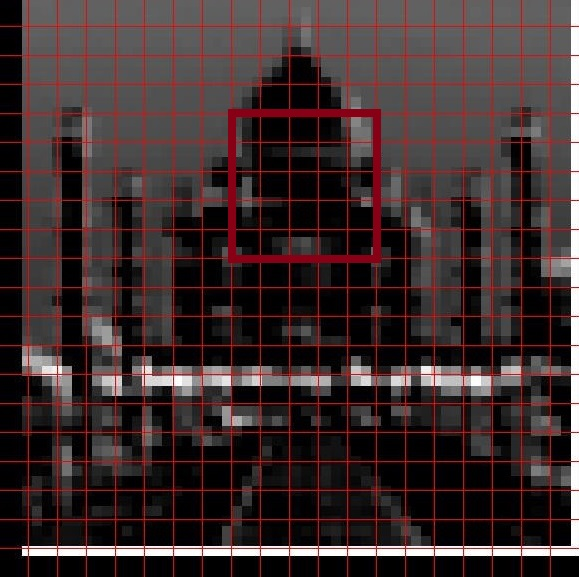
\includegraphics[width=3cm,height=2.2cm]    {images/Conv1_new.jpg}};}
	\onslide<6->{  \node[inner sep=0pt] (A) at (3,1.5)
		{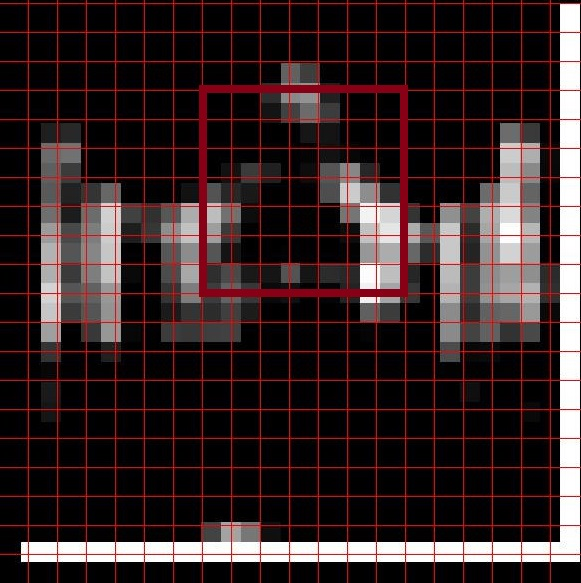
\includegraphics[width=3cm,height=2.2cm]    {images/Conv2_new.jpg}};}
\end{tikzpicture}